\documentclass[paper slide]{beamer}
\usetheme{Boadilla}
\usepackage{essay-def}
\usepackage{bm}
\usepackage{amsfonts}
\usepackage{amssymb}
\usepackage{amsmath}
\usepackage{amsthm}
\usepackage{comment}
\usepackage{subcaption}
\usepackage{geometry}
\usepackage{algorithmic}
\usepackage{algpseudocode}
\usepackage{algorithmicx}
\geometry{left=1cm,right=1cm}
    \title[Mitigating DS in SciML]{Mitigating distribution shift in machine learning-augmented hybrid fluid simulation}%\footnotemark}
\author[J. Zhao]{Jiaxi Zhao (NUS) \\ \small joint work with Sohei Arisaka and Prof. Qianxiao Li (NUS)}
\date[\today]{AMSS, CAS \\ \today}
\begin{document}
\par \setlength{\parindent}{2em}

\begin{frame}
\titlepage
%\footnotetext[1]{https://arxiv.org/abs/2401.09259}
\end{frame}


\begin{frame}{Practical scientific problems}
	%#NOTE: try to explain to the audience that these two problems are very important and subject to a lot improvement based on data-driven model
	\begin{figure}[ht]
		\centering
		\begin{subfigure}{0.5\linewidth} % Adjust the width as needed
			\centering
			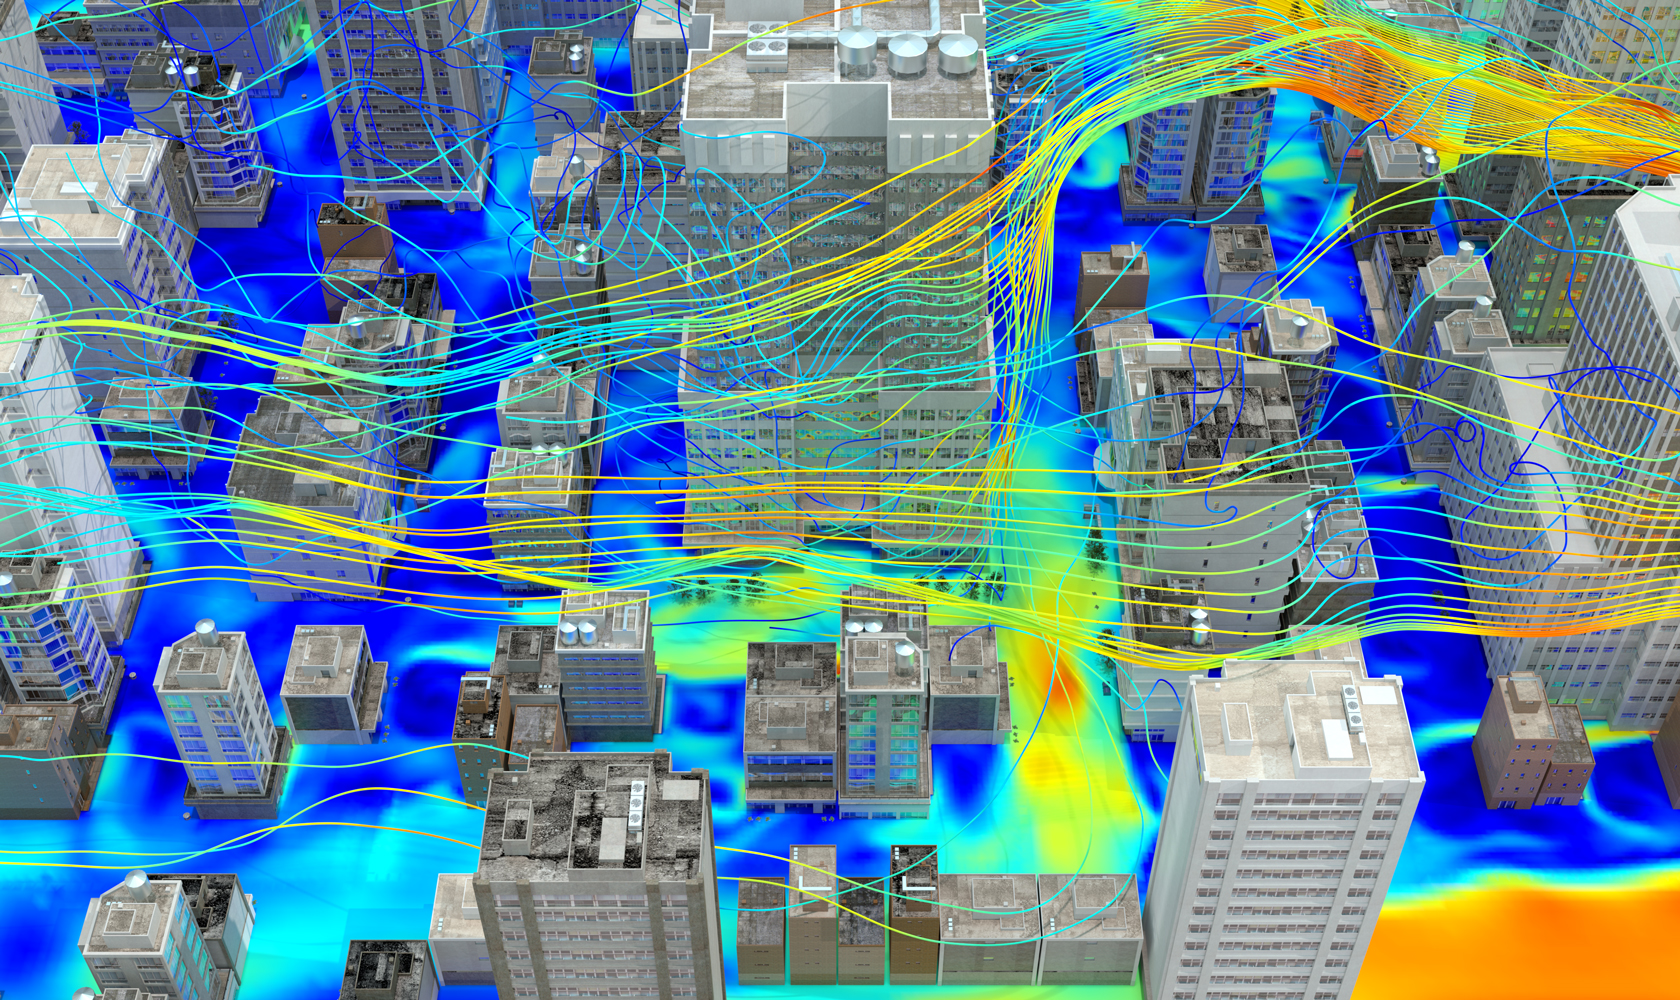
\includegraphics[width=\linewidth]{fig/urban_environment.jpeg}
			\caption{Computational fluid dynamics for urban environment}
		  \end{subfigure}%
		  \begin{subfigure}{0.5\linewidth} % Adjust the width as needed
			\centering
			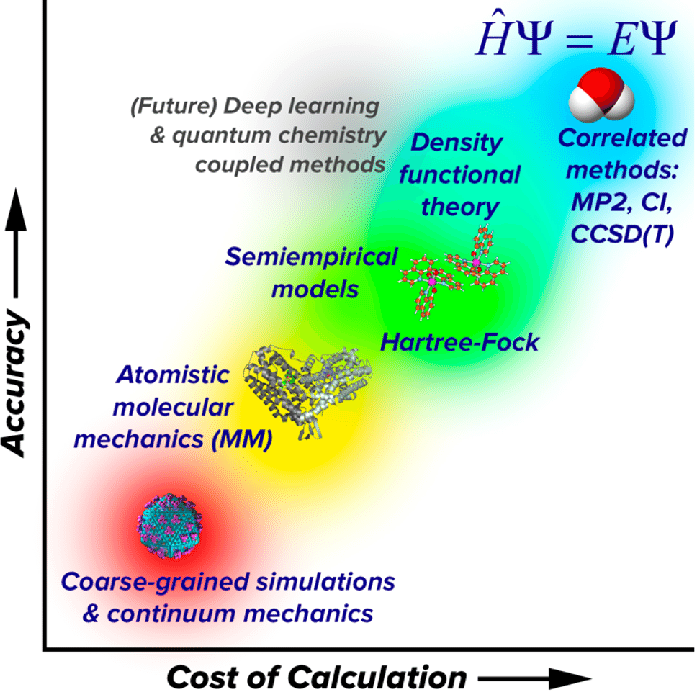
\includegraphics[width=\linewidth]{fig/quantum_chemisty.png}
			\caption{Quantum chemistry for material science}
		  \end{subfigure}
	\end{figure}
\end{frame}


\begin{frame}{Data-driven scientific computing}
	\textbf{What are the problems we are interested in?}
	\begin{itemize}
		\item 1. {\color{red}Forward problem: Increase the stability and accuracy of machine learning-augmented simulation.}
		\item 2. Inverse problem: Learn the surrogate models and Perform effective sensitivity analysis to do inverse designs. 
	\end{itemize}

	\textbf{What are methods we focus on?}
	\begin{itemize}
		\item 1. 100\% data-driven: AlphaFold series, FermiNet, Fourier neural operator, DeepONet.
		\item 2. {\color{red}50 \% Numerical + 50 \% data-driven: Machine learning turbulence modeling, force fields, exchange-correlation functionals.}
	\end{itemize}
\end{frame}

\begin{frame}{A Framework for the hybrid approach}
	Simulating the dynamics:
	\bequn
		\begin{aligned}
			\p_t \mfu & = \mcL(\mfu, \mfy, t), \quad \mfu \in \mcU, \mfy \in \mcY, \mcL: \mcU \times \mcY \times \mbR_+ \rightarrow T\mcU,			\\
			\mfy & = \phi(\mfu, t), \quad \phi: \mcU \times \mbR_+ \rightarrow \mcY.
		\end{aligned}
	\eequn
	\begin{itemize}
		\item 1. $\mcL$ is known, possibly non-linear.
		\item 2. $\phi$ is un-known.
		\item 3. A set of data pairs $\lbb (\mfu_1, \mfy_1, t_1), (\mfu_2, \mfy_2, t_2), \cdots, (\mfu_N, \mfy_N, t_N )\rbb. $
		\item 4. {\color{red}Benchmark algorithm solves the ordinary least square:
		\bequn
			\arg\min_{\theta} \mbE \norml \mfy - \phi_{\theta}(\mfu, t) \normr^2.
		\eequn}
	\end{itemize}
		{\color{red}Why surrogate models? The dynamics are unknown, nonlinear, computationally expensive etc.}
\end{frame}

\begin{frame}{An example: projection scheme}
	Let us use the incompressible NS equation as an example
	\begin{equation*}
    \begin{aligned}
        	\frac{\p \mfu}{\p t} + (\mfu \cdot \nabla)\mfu -  \nu \Delta \mfu & =   \nabla p, \quad T \in [0, 1], 	\\
		\nabla \cdot \mfu & = 0.
    \end{aligned}
\end{equation*}
Consider solving it using the projection method, in each step, we need to solve the following equation
\bequn
\begin{aligned}
	\mfu_{k+1} 	& = \mfu_k +
	\Delta t \ (\nu \Delta \mfu_k
	- (\mfu_k \cdot \nabla)\mfu_k - \nabla p_{k}),    \\
	p_{k} & = \phi(\mfu_k) = \Delta^{-1}(\nabla \cdot \lp \nu \Delta \mfu_k
	- (\mfu_k \cdot \nabla)\mfu_k\rp),   \\
\end{aligned}
\eequn

\end{frame}

\begin{frame}{An example: coarse-fine grid}
	Suppose we have a fine grid with size $2n \times 2n$ and a coarse grid with size $n \times n$.
	We want to learn a correction term between the numerical simulation in these two grid sizes.
	Fix an interpolation and a restriction operator:
	\bequn
		\begin{aligned}
			\operatorname{I}_n^{2n}: \mbR^{n \times n} \rightarrow \mbR^{2n \times 2n}, \quad \operatorname{R}_{2n}^{n}: \mbR^{2n \times 2n} \rightarrow \mbR^{n \times n}.
		\end{aligned}
	\eequn
	Now, we can state the second hybrid simulation problem as follows:
	\bequn\label{coarse-fine}
		\lbb\begin{aligned}
			\mfu_{k+1}^{2n} & = \operatorname{I}_n^{2n} \circ f_n(\operatorname{R}_{2n}^{n}(\mfu_k^{2n})) + \mfy_k^{2n},		\\
			\mfy_k^{2n} & = \phi(\mfu_k^{2n}).
		\end{aligned}\right.
	\eequn

The most important features are: 
\begin{itemize}
	\item 1. {\color{red}iterative solver}
	\item 2. {\color{red}data-driven}
\end{itemize}
\end{frame}

\begin{frame}{Dilemma of data-driven scientific computing}
	In data-driven scientific computing, \textcolor{red}{dynamics itself} can cause \textcolor{red}{distribution mismatch} between the training and testing data.
	Similarly to the \textcolor{red}{extrapolation, out-of-distribution} issue in NLP.
	\begin{figure}[ht]
		\centering
			\centering
			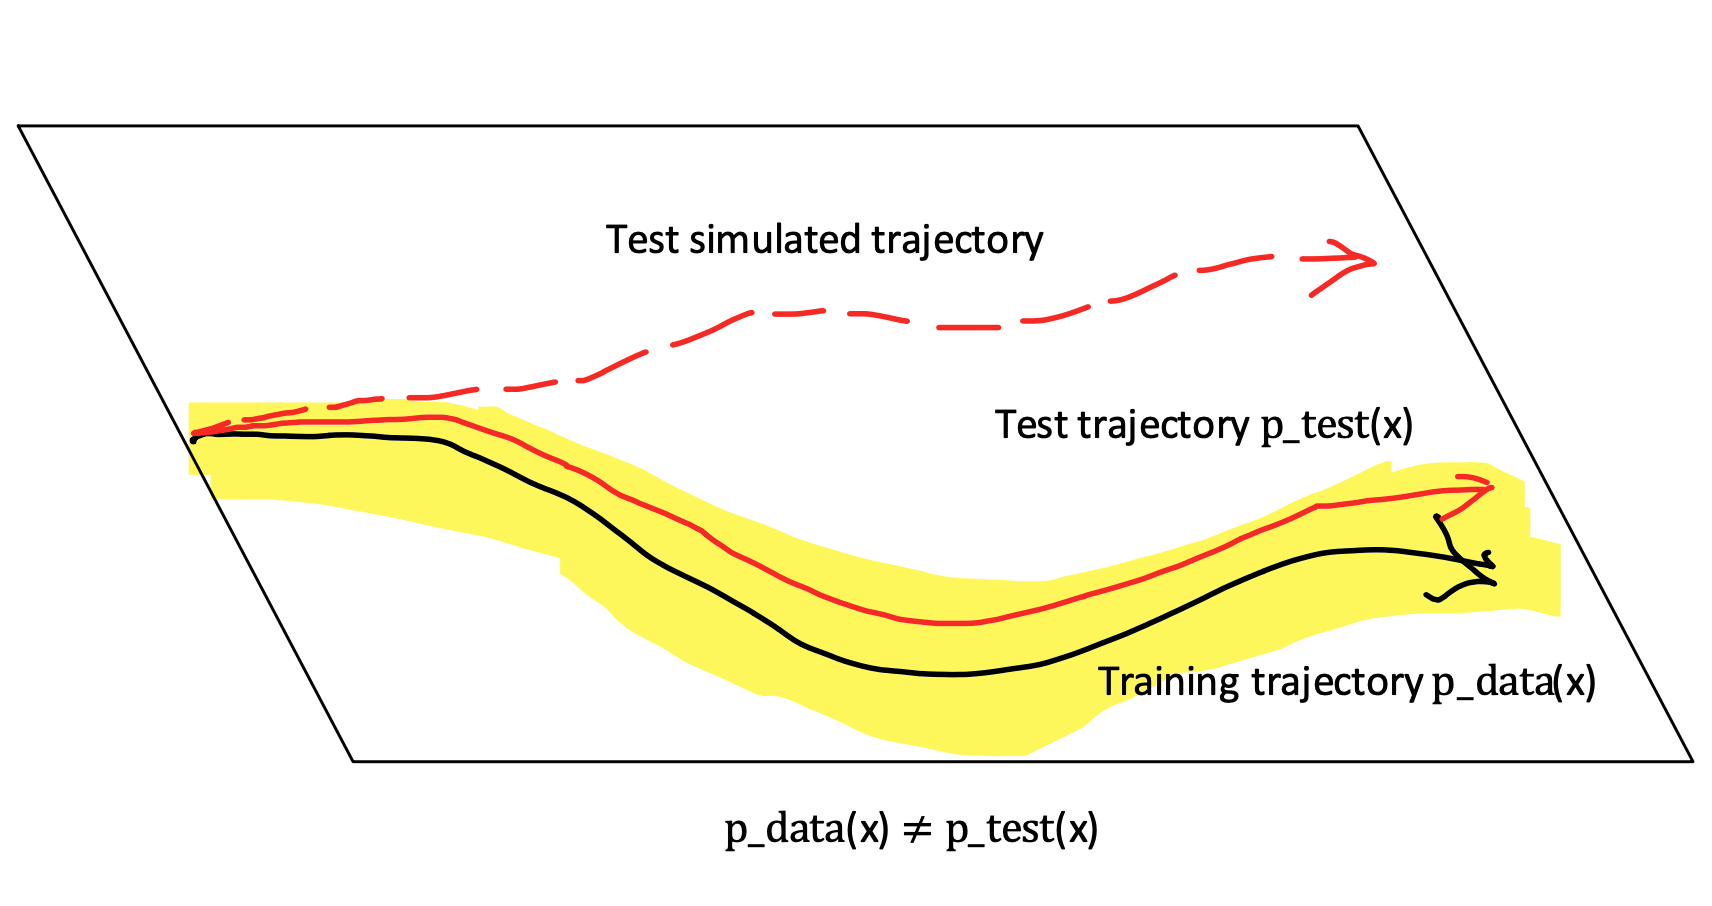
\includegraphics[width=1.1\linewidth]{fig/dilemma.jpg}
	\end{figure}
\end{frame}

\begin{frame}{Comparison with classical numerical stability}
	This is different from the classical numerical stability issue. For the ablation study, we add {\color{red}noises of the same scale to the ground truth}
	(without the data-driven part) and compare the simulations.
	\begin{equation*}
		\begin{aligned}
			\text{Data-driven model:} \quad & \phi_{\theta},	\\
			\text{Perturbed ground truth:} \quad & \phi_* + \mbE\norml \mfy - \phi_{\theta}(\mfu, t) \normr \epsilon, \ \epsilon \sim \mcN(\mathbf{0}, \mfI)
		\end{aligned}
	\end{equation*}
	where $\phi_*$ can be replaced by $\phi^{\Delta x}$, a fine-grid numerical solver.
\end{frame}

\begin{frame}{Reaction-diffusion equation}
	Consider the following FitzHugh-Nagumo reaction-diffusion equation:
	\begin{equation}
    \begin{aligned}
        	\frac{\p \mfu}{\p t} & = \gamma \Delta \mfu + \mfR(\mfu), \quad T \in [0, 1], 	\\
		\mfR(\mfu) & = \mfR(u, v) = \begin{pmatrix}
			u - u^3 - v - \alpha	\\
			\beta(u - v)
		\end{pmatrix},
    \end{aligned}
	\end{equation}
	The initial data is given by $\mfu_0$ is a random field and generated by i.i.d. sampling from a normal distribution and $\alpha = 0.001, \beta=1.0, \gamma = \begin{pmatrix}
		0.05 & 0	\\
		0 & 0.1
	\end{pmatrix}$. We use mesh size $128 \times 128$ for the whole problem. Computational domain is given by $[0, 6.4]\times[0, 6.4]$.
\end{frame}

\begin{frame}{Comparison with classical numerical stability}
	\begin{figure}[ht]
		\centering
			\centering
			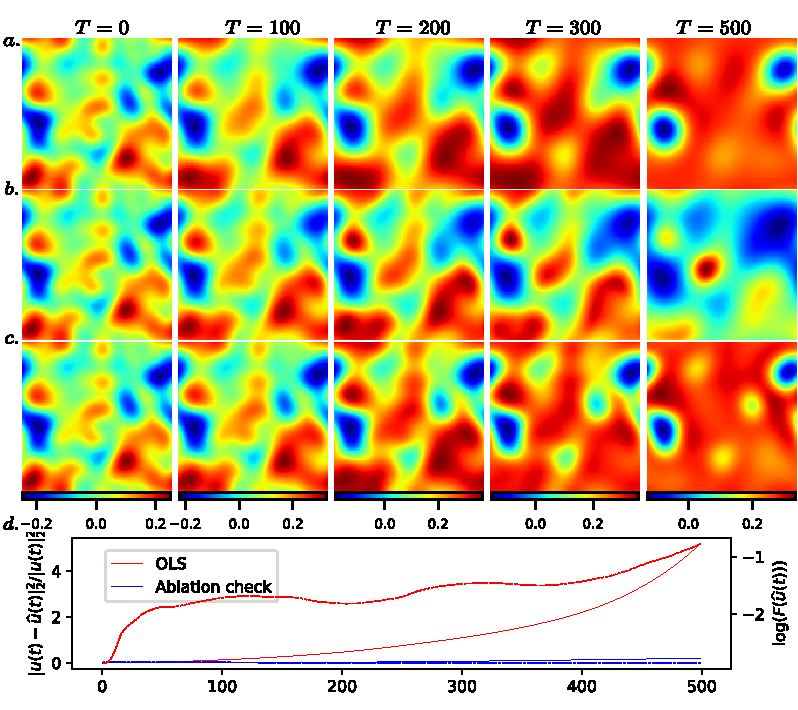
\includegraphics[width=.8\linewidth]{fig/RD-ds.pdf}
	\end{figure}
\end{frame}

\begin{frame}{An heuristic solution}
	\begin{figure}[H]
		\centering
		\centerline{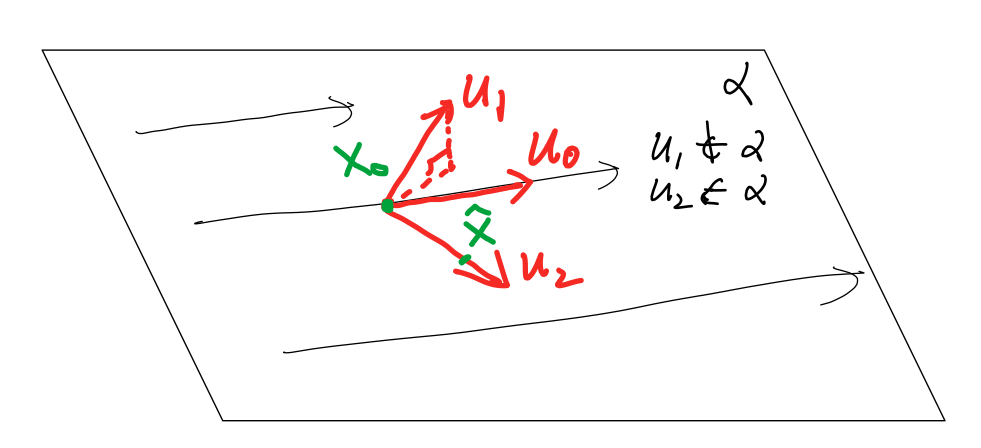
\includegraphics[width=0.8\linewidth]{fig/mfd.png}}
	  \end{figure}
	  We design an algorithm that {\color{red}favors $\mfu_2$ than $\mfu_1$} by adding some regularization.
	  This is very similar to the {\color{red}Dirac-Frenkel variational principle} in dynamical low-rank approximation.
\end{frame}

\begin{frame}{Dirac-Frenkel variational principle}
	The Dirac-Frenkel variational principle is originally developed for the Schrodinger equation 
	$\frac{d\psi}{dt} & = \frac{1}{i\hbar}H\psi$,
	\begin{equation}
		\begin{aligned}
			P\frac{d\psi}{dt} \in T_{\psi}\mcM, s.t. \la v \Big| P\frac{d\psi}{dt} - \frac{1}{i\hbar}H\psi \ra = 0, \forall v \in T_{\psi}\mcM.
		\end{aligned}
	\end{equation}
	\begin{figure}[H]
		\centering
		\centerline{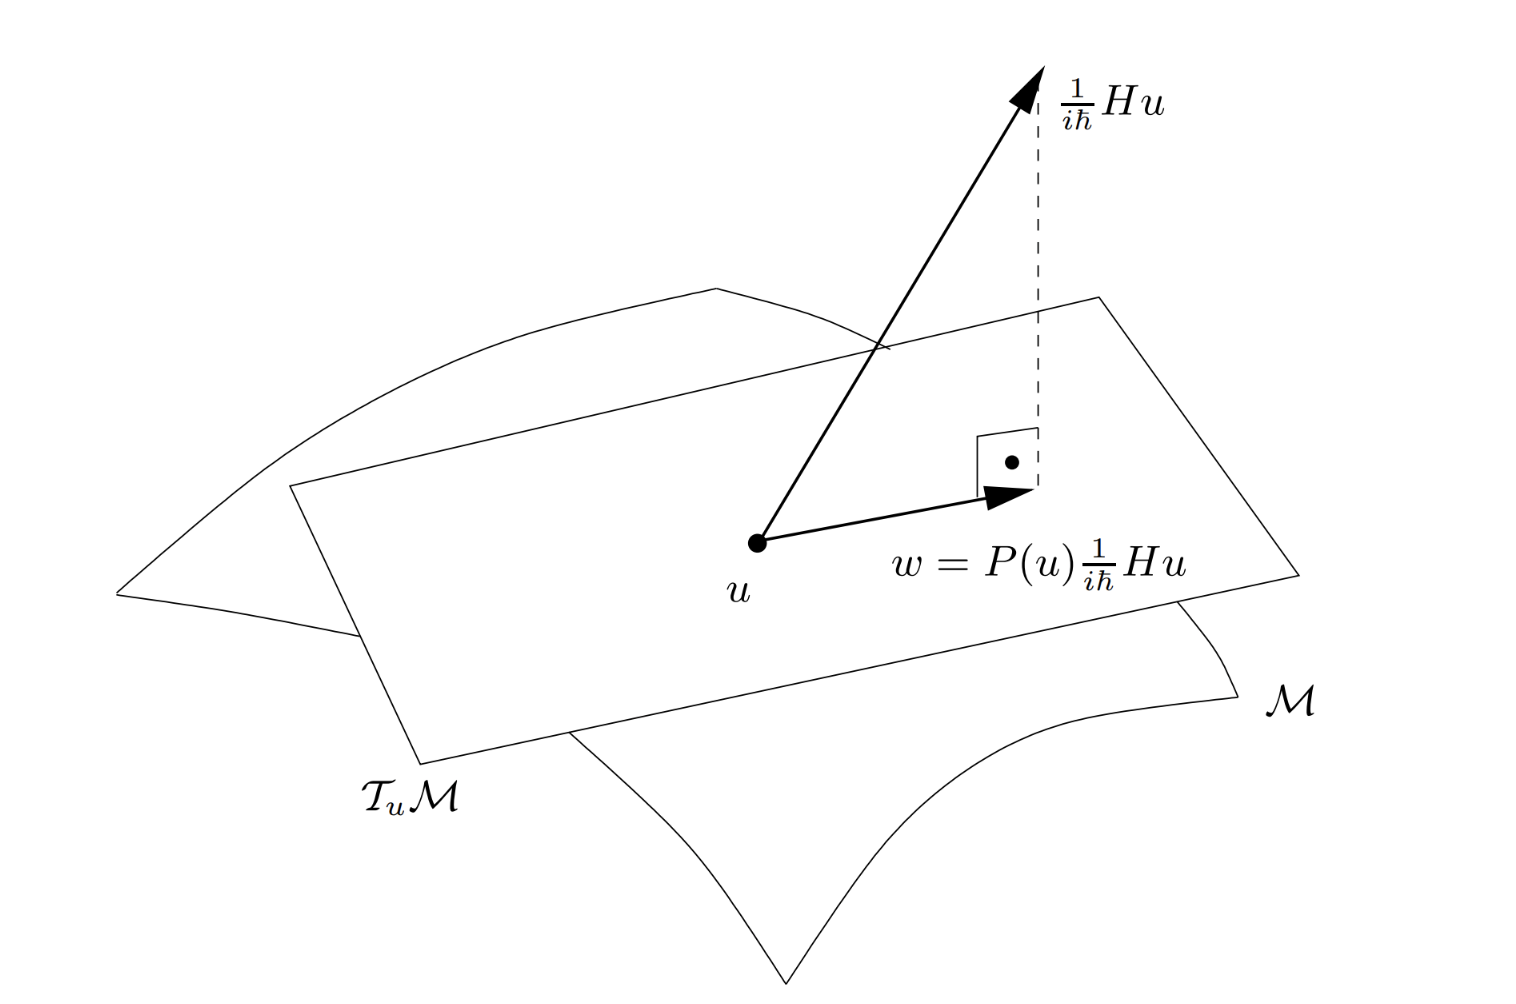
\includegraphics[width=0.6\linewidth]{fig/Dirac-Frenkel.jpg}}
	  \end{figure}
\end{frame}

\begin{frame}{Linear dynamics}
	We consider the following the \text{\color{red}linear} hybrid simulation problem
	\bequn
		\begin{aligned}
			\frac{d\mfu}{dt} & = A\mfu + B\mfy,  \quad \mfu\in\mbR^m, \mfy \in \mbR^n, A\in \mbR^{m \times m}, B\in \mbR^{m \times n}   \\
			\mfy & = C^* \mfu,  \quad C^* \in \mbR^{n\times m}.
		\end{aligned}
	\eequn
	The least squares estimator aims to minimize the following loss
	\begin{equation*}
		l_{\text{OLS}}(\wht C) = \mbE\norml (\wht C - C^*) \mfu \normr^2,
	\end{equation*}
	while the proposed estimator minimizes
	\begin{equation*}
		l_{\text{TR}}(\wht C) := \mbE_{(\mfu, \mfy)} \lp \norml (\wht C - C^*) \mfu\normr_2^2 + \lambda \norml P_{V^{\perp}}(A + B\wht C)\mfu \normr_2^2 \rp,
	\end{equation*}
\end{frame}

\begin{frame}{Linear theory}
	The tangent-space regularized estimator {\color{red}performs a weighted least squares}
	\begin{Prop}
		Given a data matrix $\mfU \in \mbR^{m \times N}$ with observation noise $\epsilon$ of the same shape 
		\begin{equation*}\label{estimator-formula}
			\begin{aligned}
			\wht C_{\text{OLS}} = & \ C^* P_V + \epsilon \mfU^{\dagger},    \\
			\wht C_{\text{TR}} = & \ (\mfI + \lambda B^T P_{V^{\perp}} B)^{-1}(C^* P_V + \epsilon \mfU^{\dagger} - \lambda B^T P_{V^{\perp}} AP_{V}).
			\end{aligned}
		\end{equation*}
	\end{Prop}
	Specifically, in the noiseless scenarios, we have
	\begin{equation*}
		\wht C_{\text{OLS}} = & \ C^* P_V, \quad \wht C_{\text{TR}} = (\mfI + \lambda P_{V^{\perp}})^{-1}(C^* P_V + \epsilon \mfU^{\dagger})= (\mfI + \lambda P_{V^{\perp}})^{-1}\wht C_{\text{OLS}}.
	\end{equation*}
\end{frame}

\begin{frame}{Linear theory}
	The tangent-space regularized estimator has {\color{red}slower error scaling for large $\lambda$}:
	%#TODO: still need to think about how to present this part
	\begin{Thm}
		With $Q_m(r, T)$ defined by $m^2\int_0^T (2 + t^{m-1})e^{r t}dt$ and
		\begin{equation*}
			\begin{aligned}
				e_1 = \text{eig}_{\max}(A+B\wht C), \quad e_2 = \text{eig}_{\max}((A+B\wht C)P_V), \\
				\text{eig}_{\max}(A) = \max\{\Re(s): \exists v \neq \mathbf{0}, Av = sv\},
			\end{aligned}
		\end{equation*}
		the errors of OLS and our algorithm are bounded respectively by
		\begin{equation*}\label{equ:a-posterior-error}
			\begin{aligned}
				& \ \mbE\norml \wht\mfu_{\text{OLS}}(T) - \mfu(T) \normr \leq c_1\sqrt{\delta}\norml B \normr_2Q_m(e_1, T),      \\
				& \ \mbE\norml \wht\mfu_{\text{TR}}(T) - \mfu(T) \normr \leq c_2\sqrt{\delta}\Big(\norml B \normr_2 Q_m(e_2, T) \\
			& + \frac{9m^4c_3}{\sqrt{\lambda}}\lp 1 + 3m^2c_1\sqrt{\delta}\norml B \normr_2\rp\norml A+B\wht C \normr_2 (1\vee T^{3m})(1\vee e^{e_1T}) \Big).
			\end{aligned}
		\end{equation*}
	\end{Thm}
\end{frame}

\begin{frame}{Linear experiments}
	Consider a linear synthetic dynamics where the data subspace $V(V^{\perp})$ is the stable (unstable) manifold.
	\begin{figure}[ht]\label{fig:linear-cmp}
		\centering
		\centerline{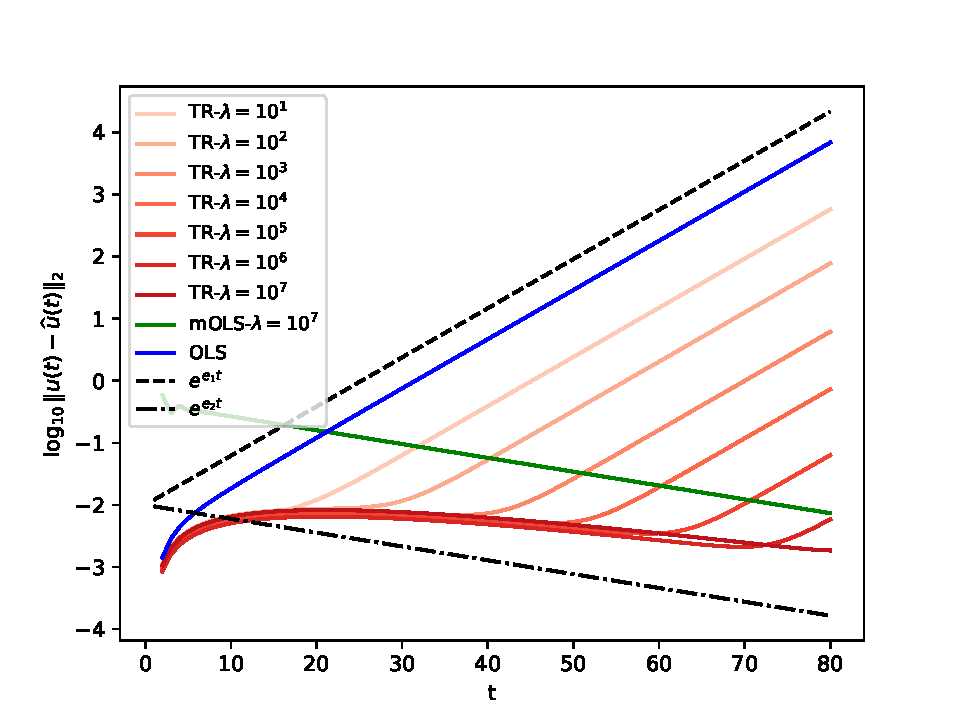
\includegraphics[width=.8\linewidth]{fig/exp2-1.pdf}}
	\end{figure}
\end{frame}

\begin{frame}{Nonlinear dynamics}
	\textcolor{red}{Use an autoencoder to parametrize the nonlinear data manifold.} We choose U-net\footnotemark as our autoencoder architecture trained via $\min_{D, E}\mbE\norml \mfu - D(E(\mfu))\normr^2$.
	Moreover, one can use $F(\mfu) = \norml \mfu - D(E(\mfu))\normr^2$ to quantify the distribution shift and $\nabla F(\mfu)$ as 
	{\color{red} a normal vector}! But there is a small caveat.
	\begin{figure}[H]
          \centering
          \centerline{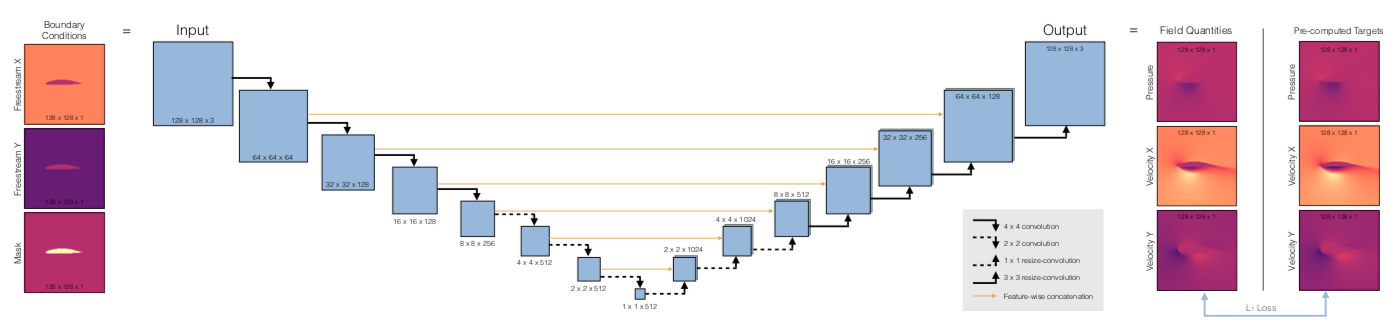
\includegraphics[width=1.1\linewidth]{fig/Unet.png}}
\end{figure}
\footnotetext{Thuerey, Nils, et al. "Deep learning methods for Reynolds-averaged Navier–Stokes simulations of airfoil flows." AIAA Journal 58.1 (2020): 25-36.}
\end{frame}

\begin{frame}{Overall algorithm}
	%#TODO: the algorithm itself is hard to present, think about how to simplify it
	\begin{figure}
		\centering
		\centerline{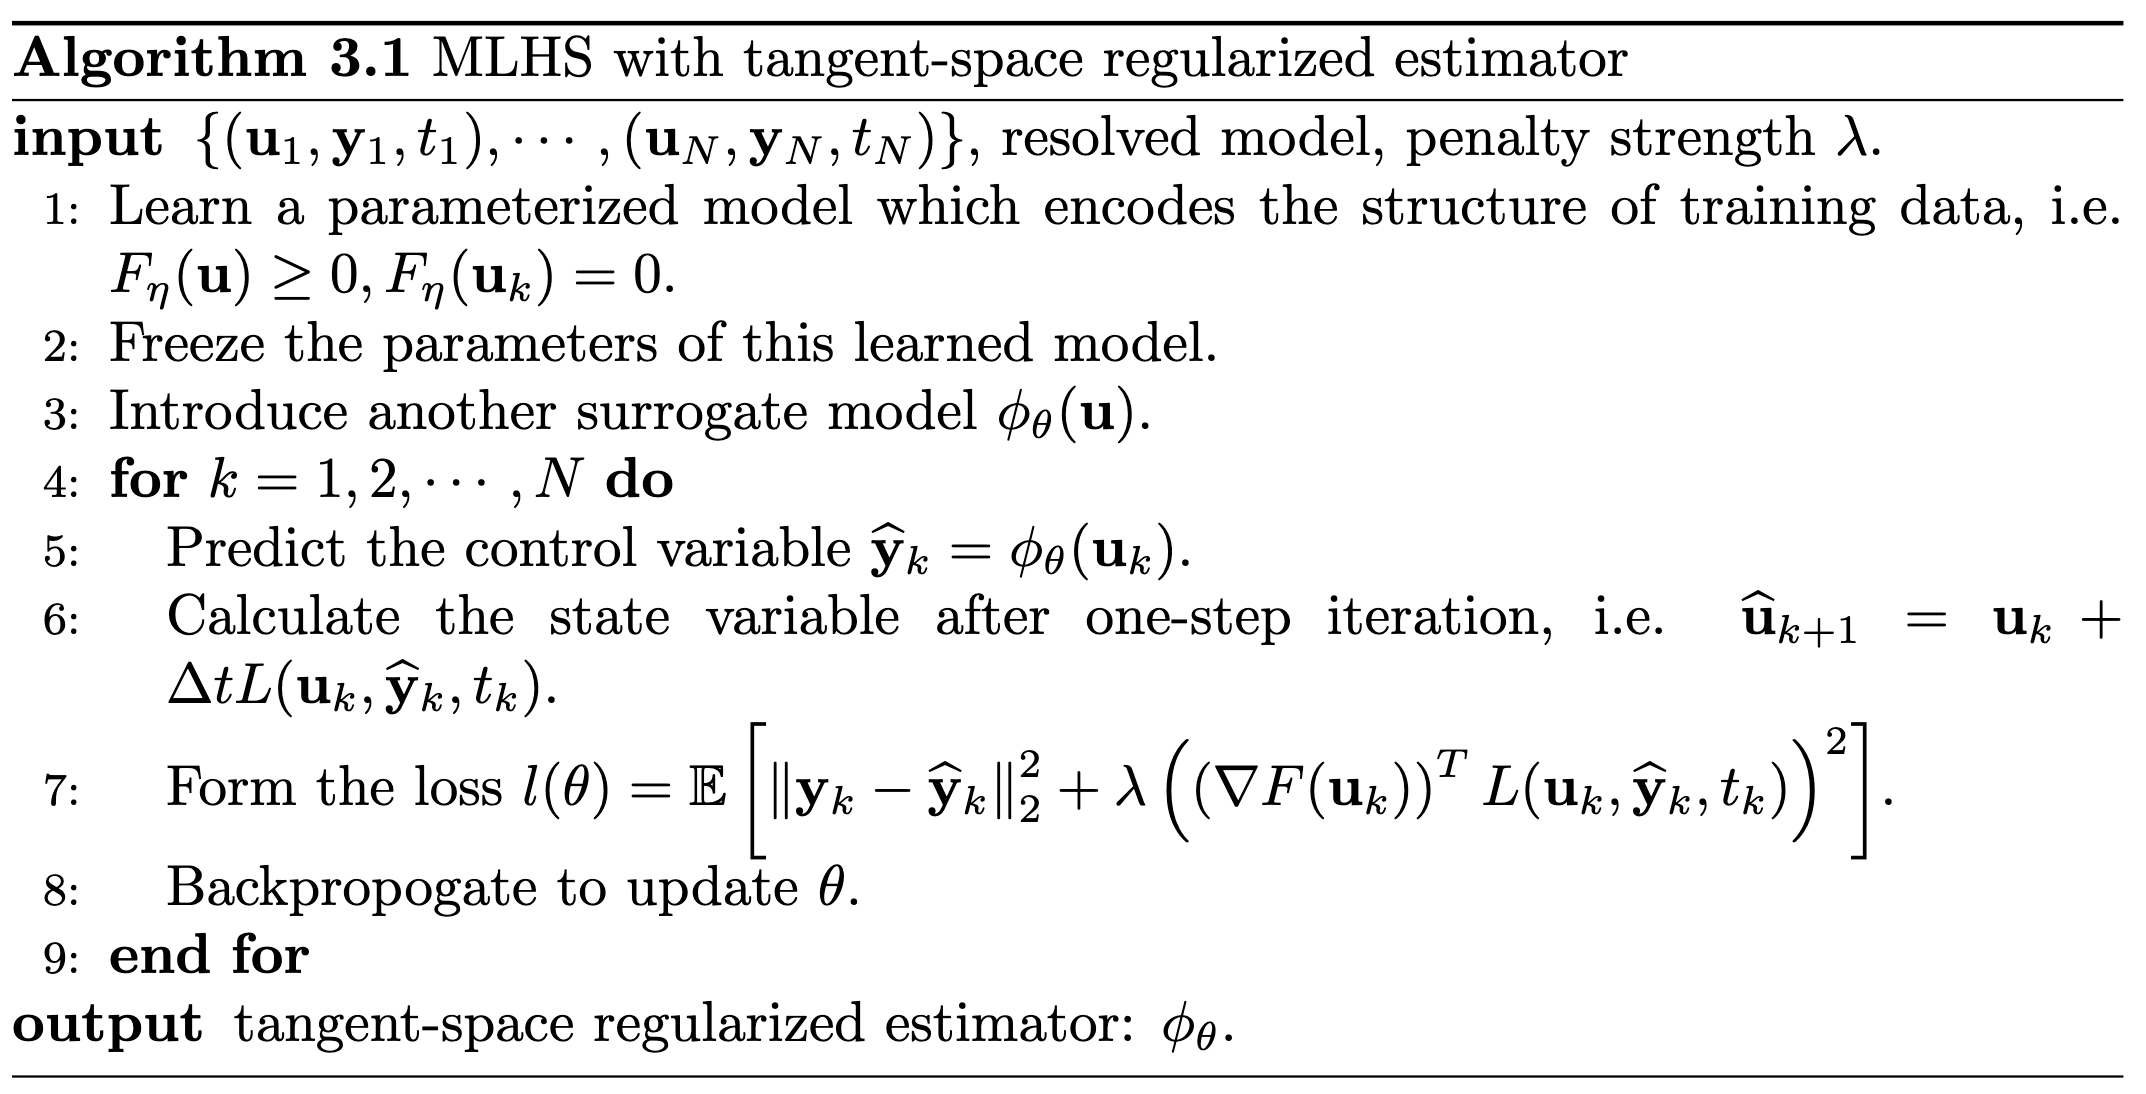
\includegraphics[width=\linewidth]{fig/alg.jpg}}
	\end{figure}
	{\color{red} Our method is non-intrusive.}
\end{frame}

\begin{frame}{Performance comparison}
	\begin{figure}[H]
          \centering
          \centerline{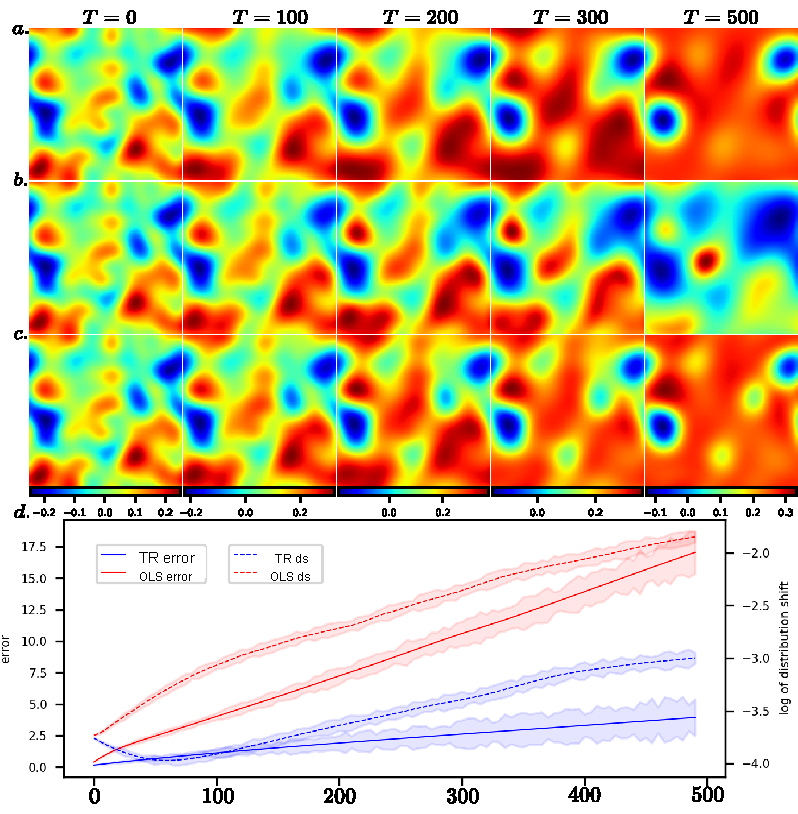
\includegraphics[width=.75\linewidth]{fig/RD-TR.pdf}}
\end{figure}
\end{frame}

\begin{frame}{Performance comparison}
	\begin{figure}[H]
          \centering
          \centerline{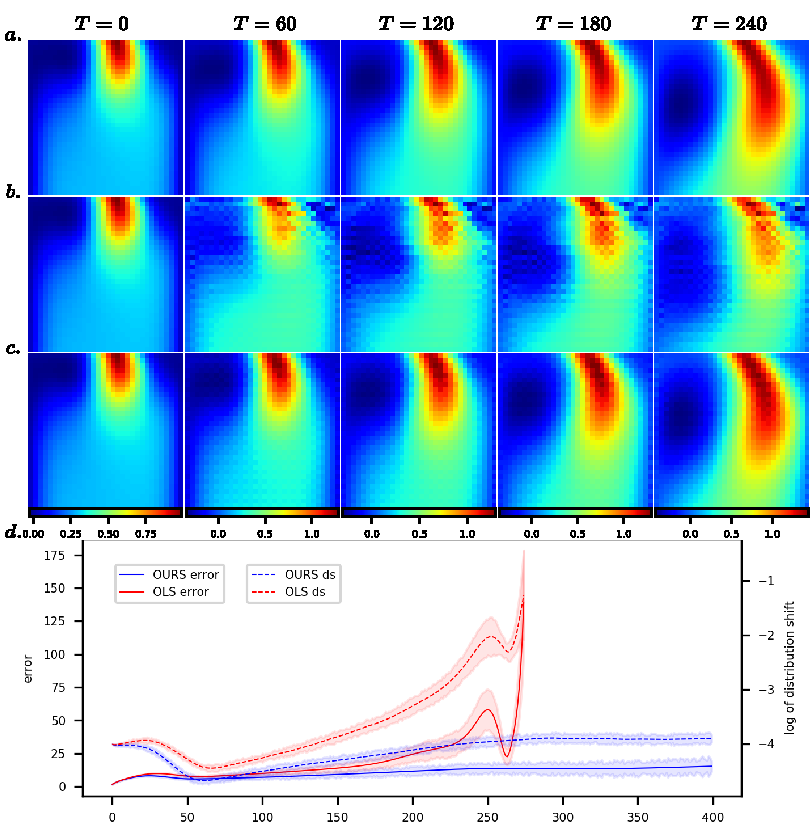
\includegraphics[width=.75\linewidth]{fig/NS-TR.pdf}}
          \caption{Comparison of our method and naive method}
\end{figure}
\end{frame}

%%%%%%%%%%%%%%%%%%%%%%%%%%%%%%%%%%%%%%%%%%%%%%%%%%%%%%%%%%%%%%%%%%%%%%%%%%%%%%%%%%%%%%%%%%%%%%%%%%%%%%%%%%%%%%%%
%    below starts the discussion on the LES project
%%%%%%%%%%%%%%%%%%%%%%%%%%%%%%%%%%%%%%%%%%%%%%%%%%%%%%%%%%%%%%%%%%%%%%%%%%%%%%%%%%%%%%%%%%%%%%%%%%%%%%%%%%%%%%%%
\begin{frame}{Subgrid-scale stress modeling based on NN}
	\begin{equation*}
		\begin{aligned}
		\frac{\p \overline{u}_i}{\p t} + \frac{\p}{\p x_j}(\overline{u}_i\overline{u}_j) & \ = -\frac{\p \overline{p}}{\p x_i} + \nu\Delta \overline{u}_i - \frac{\p \tau_{ij}}{\p x_j},   \\
		\frac{\p \overline{u}_i}{\p x_i} & \ = 0.
		\end{aligned}
	  \end{equation*}
	\begin{itemize}
		\item 1. Performing DNS is unaffordable, even a LES with 50M grids of length 1000s takes several days.
		\item 2. Cheap simulations such as RANS and coarse-grid LES can not obtain accurate quantities such as peak pressure.
	\end{itemize}
	\textit{Can we {\color{red}design or learn better SGS models} based on the LES data so that it can achieve accurate
	results even {\color{red}on coarse grid LES?}}
\end{frame}

\begin{frame}{SGS stress modeling}
	There are three main issues for stress modeling:
	\begin{itemize}
		\item 1. The mapping from the input features. e.g. filtered velocity to the stress tensor is {\color{red}non-deterministic} while
		most classical turbulence models and data-driven models are deterministic.
		\begin{equation*}
			\overline{\mfU}, \nabla \overline{\mfU}, \overline{p} \overset{\text{NOT DETERMINISTIC}}{\Longrightarrow} \tau, \quad \min_{\phi}\norml \tau - \phi(\overline{\mfU}) \normr^2.
		\end{equation*}
		\JX{We could try to mention that we can include a larger region of the
		filtered information so that the mapping may become deterministic.}
		\item 2. The discrepancy between {\color{red}a-priori error and a-posteriori error}.
		\begin{equation*}
			\norml \wht\tau - \tau \normr^2, \quad \norml \overline{\wht\mfU}(T) - \overline{\mfU}(T) \normr^2
		\end{equation*}
		\item 3. Difficult to combine the OpenFOAM solver with gradient-based optimization algorithms.
	\end{itemize}
\end{frame}

\begin{frame}{Learning the SGS stress model}
	We test the following three approaches:
	\begin{itemize}
		\item 1. {\color{red}Directly predict} the stress tensor from the input features.
		\begin{equation}
			\tau = \text{NN}(\overline{\mfU}, \nabla \overline{\mfU}, \overline{p}).
		\end{equation}
		\item 2.  {\color{red}Learn a correction} of the constants to the Smagorinsky model.
		\begin{equation}
			\wtd C = \text{NN}(\overline{\mfU}, \nabla \overline{\mfU}, \overline{p}) + C, \quad \nu_t = \wtd C \Delta^2 \lv \bar{S} \rv.
		\end{equation}
		\item 3. Learn a  {\color{red}conditional generative model} from the input features.
	\end{itemize}
	\begin{itemize}
		\item The first approach usually provides a much better a-priori error estimate than the second approach.
	\end{itemize}
\end{frame}

\begin{frame}{Probabilistic SGS stress modeling}
	While the first two deterministic stress models can not capture the statistical behavior of the SGS stress,
	our probabilistic stress model manages this:
	\begin{figure}[ht]
		\centering
		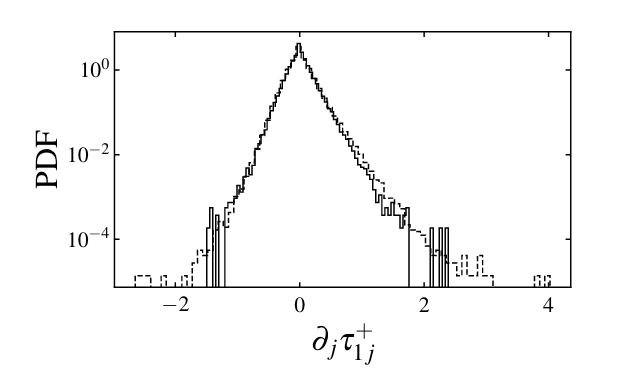
\includegraphics[width=.6\linewidth]{fig/stress_hist.jpg}
	\end{figure}
	\begin{figure}[ht]
		\centering
		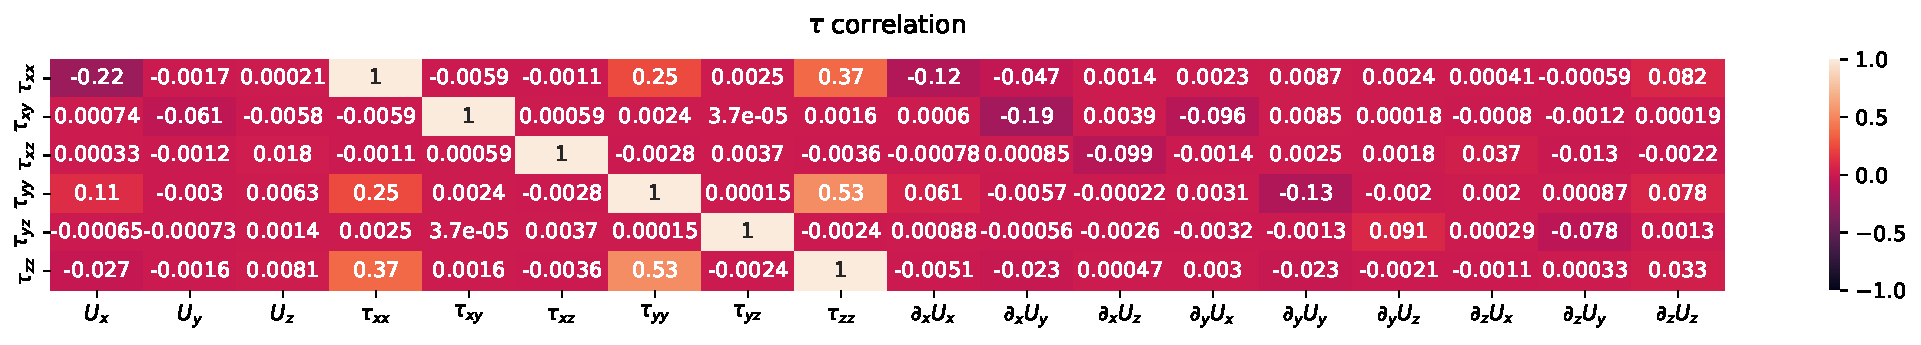
\includegraphics[width=1.2\linewidth]{fig/heatmap_tau.pdf}
	\end{figure}
\end{frame}

\begin{frame}{A-priori and a-posteriori discrepancy}
	The inconsistency between the a priori error and a posteriori error arises because the {\color{red}training algorithm does not take the solver dynamics into account}.
	\begin{figure}
		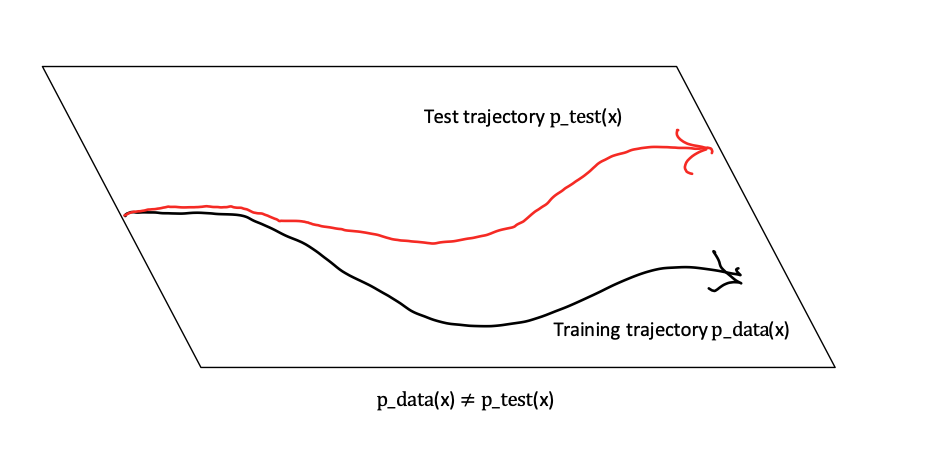
\includegraphics[width=.6\textwidth]{fig/dilemma.png}
		\label{fig:dilemma}
	\end{figure}
	The a-priori and a-posteriori performance are not consistent.
	\begin{figure}
		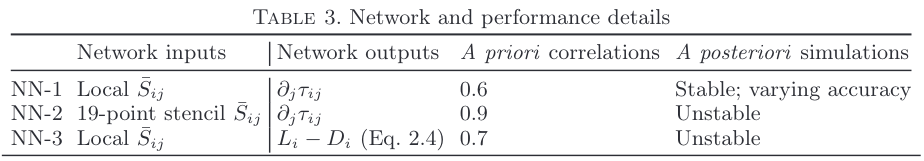
\includegraphics[width=.8\textwidth]{fig/dichotomy.jpg}
		\label{fig:dichotomy}
	\end{figure}
\end{frame}

%TODO: this is not my contribution, try to modify this, we may directly delete this part
\begin{comment}
\begin{frame}{Problem: Non-automatic-differentiable Solver}
    To directly minimize a posteriori error,
    we need to incorporate OpenFOAM solvers into the neural network training.
 
    However, they are not automatic-differentiable,
    and computing gradients through them is not trivial.
 
    \begin{figure}
        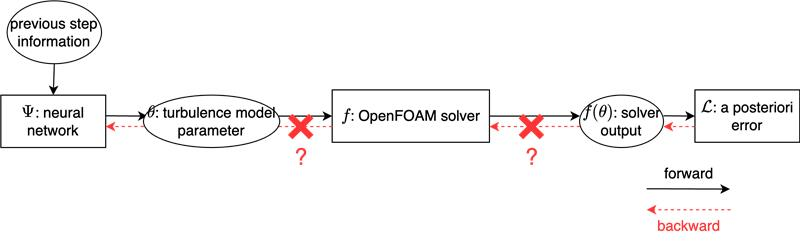
\includegraphics[width=\linewidth]{fig/of_problem.jpg}
    \end{figure}
    
\end{frame}
 
\begin{frame}{Solution: Non-intrusive Wrapper}
    To enable joint training with neural networks and such solvers,
    we developed a non-intrusive methodology that wraps the solvers
    to be compatible with neural network training.
 
    The key idea\footnotemark is to construct an unbiased and low-variance gradient estimator
    using a surrogate model that mimics the solver's behavior.
 
    \begin{figure}
        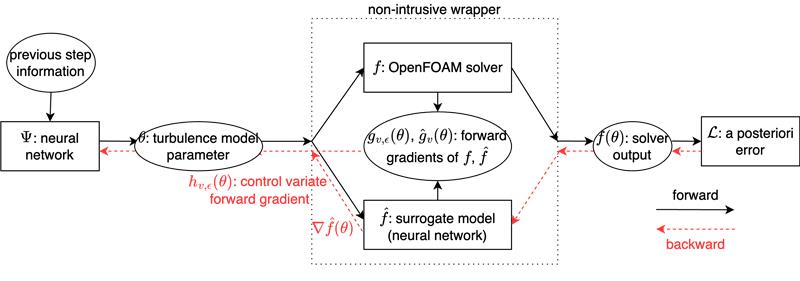
\includegraphics[width=\linewidth]{fig/of_solution.jpg}
    \end{figure}
    \footnotetext{S. Arisaka and Q. Li (2024) Accelerating Legacy Numerical Solvers by Non-intrusive Gradient-based Meta-solving}
    
\end{frame}


\begin{frame}{Preliminary result}
    We have applied the methodology to PETSc linear solver for Poisson equations by learning initial guesses
    and reduced the number of iterations by 74\%.
 
    We plan to apply it to learning turbulence models in OpenFOAM beyond linear solvers.
 
    \begin{figure}
        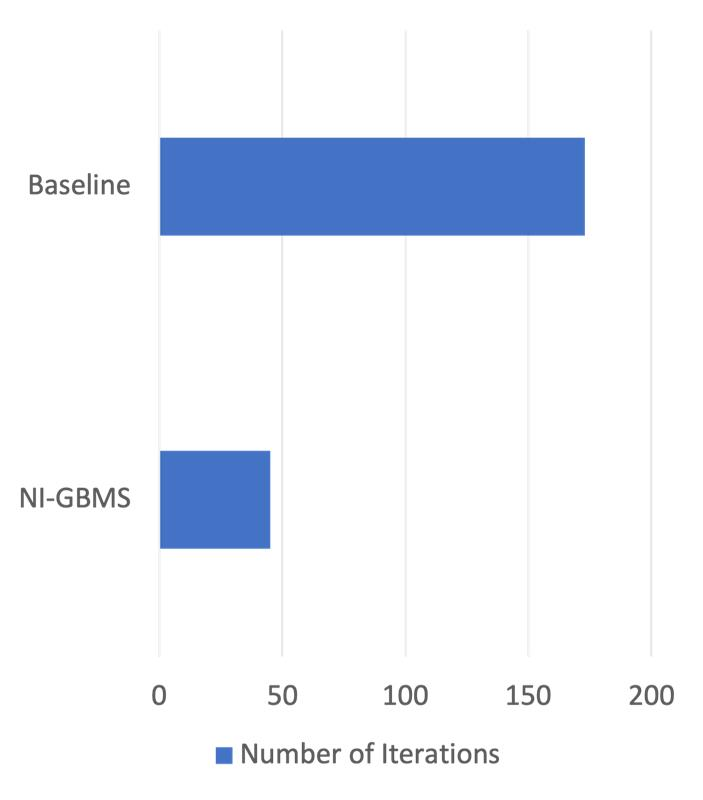
\includegraphics[width=0.4\linewidth]{fig/poisson_eq.jpg}
    \end{figure}    
    
\end{frame}
\end{comment}
 
\begin{frame}{Dateset preparation and preprocessing}
	Judging the quality of the dataset is crucial for our application, which is also very different from
	the numerical PDE cases as grid convergence tests are inapplicable.
	\begin{figure}
        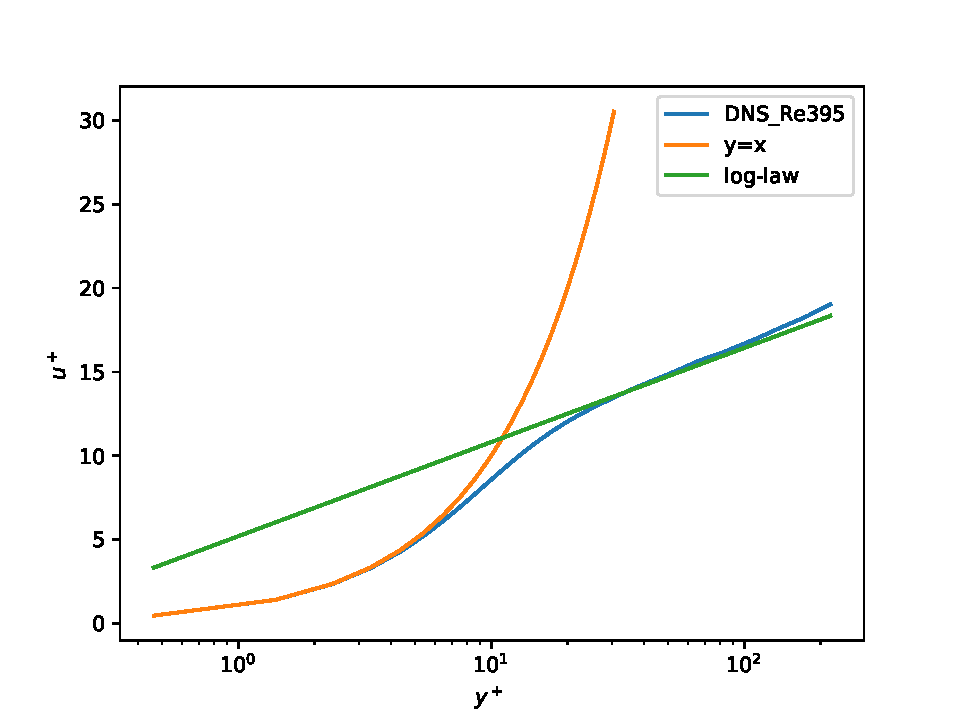
\includegraphics[width=0.7\linewidth]{fig/velocity_profile.pdf}
    \end{figure}    
\end{frame}

\begin{frame}{Future work}
	\begin{itemize}
		\item 1. Generate a systematical dataset of the flow around bluffs; train SGS models within the dataset and design algorithms
		which improves the a-posteriori performance.
		\item 2. Deploy to practical problems: Subgrid-scale modeling in large eddy simulation of the
		urban environment.
		\item 3. Investigate the statistical and numerical properties of the data-driven turbulence modeling, with
		special focus on the dataset characteristic and the relation between data with different resolutions.
	\end{itemize}
\end{frame}

\begin{frame} % Use [allowframebreaks] to allow automatic splitting across slides if the content is too long
    \frametitle{References}
 
    \begin{thebibliography}{99} % Beamer does not support BibTeX so references must be inserted manually as below, you may need to use multiple columns and/or reduce the font size further if you have many references
        \footnotesize % Reduce the font size in the bibliography
 
		\bibitem[BDI]{bdi}
		M. Benjamin, S. Domino, and G. Iaccarino
		\newblock Neural Networks for Large Eddy Simulations of Wall-bounded Turbulence: Numerical Experiments and Challenges
		\newblock \emph{The European Physical Journal E}

		\bibitem[Zhao 2024]{ds}
        J. Zhao and Q. Li (2024)
        \newblock Mitigating Distribution Shift in Machine Learning-augmented Hybrid Simulation
        \newblock \emph{Arxiv preprint https://arxiv.org/pdf/2401.09259}

        \bibitem[S.A. and Q.L., 2024]{nigbms}
        S. Arisaka and Q. Li (2024)
        \newblock Accelerating Legacy Numerical Solvers by Non-intrusive Gradient-based Meta-solving
        \newblock \emph{International Conference on Machine Learning 2024}
 
        
    \end{thebibliography}
\end{frame}

\end{document}